\documentclass{article}
\usepackage{graphicx}
\usepackage{amsmath}
%\usepackage{algorithmic}
%\usepackage{algpseudocode}
%\usepackage{algpascal}
\usepackage{url}
\usepackage{hyperref}
\usepackage[letterpaper, margin=1.5in]{geometry}
\geometry{
 a4paper,
 total={170mm,257mm},
 top=20mm,
 }
 \graphicspath{ {images/} }

\begin{document}

\title{\textbf{Flappy Bird Game AI using Neural Networks}}
\author{Aviral Kumar, 140070031 \\Saurabh Garg, 140070003\\ Siddhant Garg, 14D070027\\ Ritwick Chaudhry, 14D070063 }

\maketitle
\begin{center}
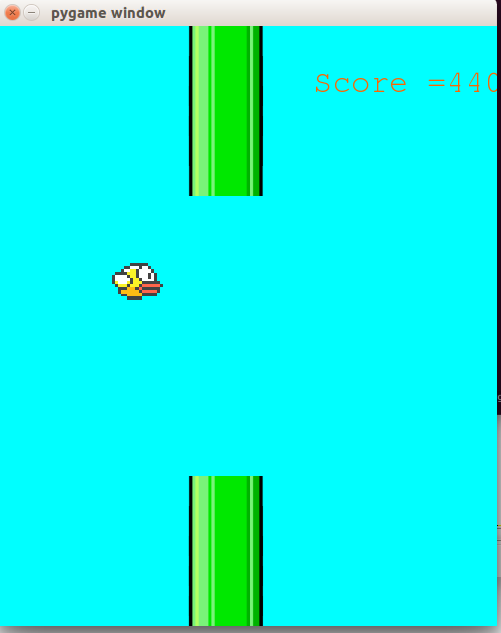
\includegraphics[width=0.35\vsize, angle = 0]{screenshot.png} \\
\end{center}
\pagebreak
\tableofcontents
\pagebreak

\section{Abstract}
Genetic Algorithms and Reinforcement Learning are useful for finding solutions to problems for which there is no clear solution and the situations vary with time, i.e. for probabilistic situations. In this project, we have implemented an AI for the Flappy Bird which makes the computer play the game much more efficient as compared to what a normal human being can do. We have achieved these goals using Genetic Algorithms with an underlying Neural Network Architecture.

\section{Proposed Idea}
We had originally proposed to create an AI for the Flappy Bird Game, which can learn how to play the game optimally, all by itself using Deep Q Learning, which is a type of reinforcement learning. Due to some time and knowledge constraints we realised that we were not on track to finish this, so after discussions with and based on the recommendations of the Mentors, we made some small changes to the project. Instead of using Reinforcement Learning, we have now used \textbf{Genetic Algorithms} to solve the problem. The project still involves a Neural Network at its backend. The original problem remains the same even now. The apporach towards it has been changed.   

\section{Introduction}	

The main aim of this project is to develop a Genetic Algorithm based approach for constructing an AI which can play the Flappy Bird game much more efficient as compared to a normal human being.
\hfill \break
\hfill \break
Flappy Bird is a game where the player tries to make the bird cross the maximum number of pillars while it's alive. If the bird hits any pillar, or the ground, it dies and the game ends. Pillars can come up randomly and can have variable heights. The player has 2 moves : first, to make the bird move up, and the second to not do anything, and consequently let the bird fall downwards to the ground. The player tries to navigate the bird safely through the maximum possible number of pillars. Each pillar crossed successfully adds 1 to the score.
\hfill \break
\hfill \break
\textbf{Genetic Algorithms} are adaptive heuristic search algorithms based on the evolutionary ideas of natural selection and genetics. As such they represent an intelligent exploitation of a random search used to solve optimization problems. Although randomised,these are by no means random, instead they exploit historical information to direct the search into the region of better performance within the search space. The basic techniques of these are designed to \textbf{simulate processes in natural systems} necessary for evolution, specially those follow the principles first laid down by Charles Darwin of \textbf{survival of the fittest}. Since in nature, competition among individuals for scanty resources results in the fittest individuals dominating over the weaker ones.(\url{https://www.doc.ic.ac.uk/~nd/surprise_96/journal/vol1/hmw/article1.html})
\hfill \break
\hfill \break
Genetic Algorithms allow us to explore a space of parameters to find solutions that score well according to a \textbf{fitness function}. They are a way to implement function optimization: given a function g(x) (where x is typically a vector of parameter values), find the value of x that maximizes (or minimizes) g(x).(\url{http://theory.stanford.edu/~amitp/GameProgramming/AITechniques.html})

\section{Motivation}

We had seen videos of Genetic Algorithm based Approaches applied to solving optimization problems, mostly games like MarI/O (\url{https://www.youtube.com/watch?v=qv6UVOQ0F44}) , Attari Deep Mind, etc. We were quite influenced by these approaches and hence we decided to implement a similar thing on the Flappy Bird Game, as it is not much of a complicated game, and hence apt for beginners like us. Hence, we decided to make an AI for this game using two main concepts of : \textbf{Genetic Algorithms} and \textbf{Neural Networks}.

\section{Theory behind Genetic Algorithms}

Genetic Algorithms mimic the survival of the fittest, in a way that, generations are maintained, and from one generation, only those characters are able to pass to the next generation which have survived/performed well in that generation. Each generation is characterised by a set of strings, which are analgous to the chromosomes in the DNA. Cross-Over, Mutations and other biological effects occur and in turn affect the offspring in the next generation. The same holds true for a genetic algorithm too. Each individual represents a point in a search space and a possible solution. The individuals in the population are then made to go through a process of evolution.
\hfill \break
\hfill \break
In biology, individuals compete for resources, some of them win and others lose. The winning individuals are likely to contribute more share to the offspring as compared to the losing ones. Offspring inheriting features from two winning individuals has a good chance of being better than each of its parent. The logic remains the same her also. Some of the important terms related to Genetic Algorithms are explained below:  

\subsection{Search Space}

A set of individuals is maintained within a search space. Each individual represents a candidate solution to a problem(in our case, this is weights of the edges in the Neural Net). Each individual is coded as a string representing it. (The Weight vector coverted to string) (Individuals are like chromosomes, and the entries in that vector representing an individual are like genes. The fitness function which was mentioned earlier defines the competing ability of an individual. The aim is to make the offspring produced by this generation iherit the best properties of any two individuals from this generation.

\subsection{Selection}

In the biologic analogy, the "fittest" individual is chosen to be passed on to the next generartion. In our implementation too, the individuals with the top 5 fitness values pass on to the next generation without any hinderance. 

\subsection{Cross Over}

Two indviduals are selected from a generation and a position in their bit strings is chosen at random. The bits corresponding to this position are swapped between the too. Now, this offspring also passes on to the nest generation. As this combines good individuals too, it has a fiarly likely chance of showing up an individual which is better than the current generation. 

\subsection{Mutation}

This happens very rarely, ths bits of some people are flipped at some randomly chosen position. This ensures that the solution doesn't converge to an answer which is not globally optimal, and that there is always a chance to revert back, and not converge to a wrong point. 

\section{Our Implmentation}

\textbf{Neural Network: }We have formed a Neural Network with two input nodes, one for the distance of the bird from the closest vertical pipe and the second for the height of the bird from the vertical level of the closest pipe. There is one hidden layer with 2 nodes and an output layer with 1 node. Each node uses the sigmoid function as its activation function. \hfill \break
\hfill \break
\textbf{Inputs :} The horizontal distance of the bird from the next pair of pipes ($x_{next}$), The height of the bird above the top of the lower of the next pipes to be encountered ($h$).
\hfill \break \hfill \break
\textbf{Outputs :} A single value, if $\geq$ 0.5 , it means perform flap and else do nothing.
\hfill \break
\hfill \break

\textbf{Individual:} So, there are 6 weights ( 4 from the IL to the HL and the remianing two from the HL to the OL). A string formed by concatenating all the weight values and encoding it into a string, reprsents an individual in the current generation.
\hfill \break
\hfill \break

\textbf{Fitness Parameter: }The fitness parameter for our implementation is the weighted average of the score of the bird in the game and the distance to which it has moved. Keeping distance a parameter in the fitness function is important so that two positions of the bird between two consecutive pillars can be distinguished. It also ensures, in the long run, that the bird moves a larger distance instead of staying at the same place and ensures faster convergence.
\hfill \break
\hfill \break
\textbf{From one generation to the next :} We have implemented a function that goes by the name \textbf{breed()}, in which we first sort the individuals of the current generation in decreasing order of their fitness values, then the top 5 ones are directly passed on to the next generation. Also, we divide the 20 individuals in each layer into groups of 2, and cross the two falling in one pair. Then their children are mutated and passed on to the next generation.  


\section{Finer Code level Details}
\begin{enumerate}
    \item The code is run by executing the \texttt{newgen.py} file, which inturn calls the other sub modules.
    \item We have used pygame, numpy, math and random libraries of python for implementing ths stuff.
    \item As the execution begins, a new random neural network is initialised, and then it control loops through n generations, each time updating the individual set, and displaying the best result of that generation by an instance of the game.
    \item The file newgen.py has 4 main functions : performance(), updateweights(), survivaloffittest() and newnetlist(). 
    \item The \textbf{performance()} function returns an instance of the game where the bird actually plays the game.
    %\item The \textbf{mutate()} function takes the genome (string representation), chooses a bit randomly , and then changes it using the random triangular distribution, and finally returns this modified gene.
    \item The \textbf{survivalofthefittest()} function considers the two topmost entries of the genome and then returns the one the maximum fitness level.
    \item The \textbf{updateweights()} function combines them all into one function. Children are formed from the current generation by crossing over the two parents. Along with this, some of these children suffer random mutations (only some of these, as the condition of the if statement corresponds to an inequality with the \textbf{mutationrate}, which might not be satisfied always), and then they get passed on as the individuals of the next generation.
    \item The function \textbf{newnetlist()} takes in the genome of generation i and then takes  two individuals in pairs from the sorted genome in decreasing order of fitness, breeds them and returns the result as the individuals of generation (i+1)
    \item The file \texttt{newgen.py} also corresponds to the implementation of the underlying Neural Net class on which the entire computation is being done. It has two new functions apart from the common neural net, which are : \textbf{nettolist() and listtonet()}. These are used to convert the weight vector back to and convert to weight vector back from, the string representing the weight array (individuals).
    \item The file \texttt{flappygame.py} is used to create the basic GAME UI which has been referenced from the link mentioned specifically in the references. 
\end{enumerate}

\section{Observations}
We ran the code for about 20 generations, and found out the maximum score the bird reached.
This is depicted in the graph shown below.
\begin{center}
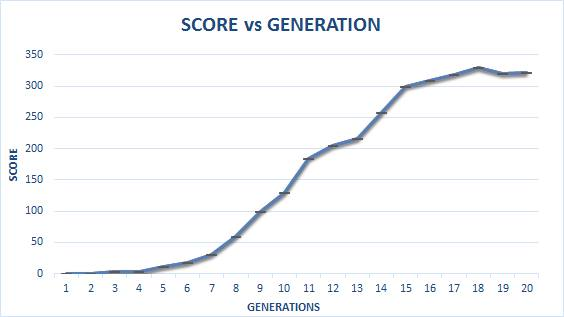
\includegraphics[width=0.5\vsize, angle = 0]{graph.png} \\
\end{center}
A screenshot of the bird, after it hits the pipe at a Score of 557 is shown below:
\begin{center}
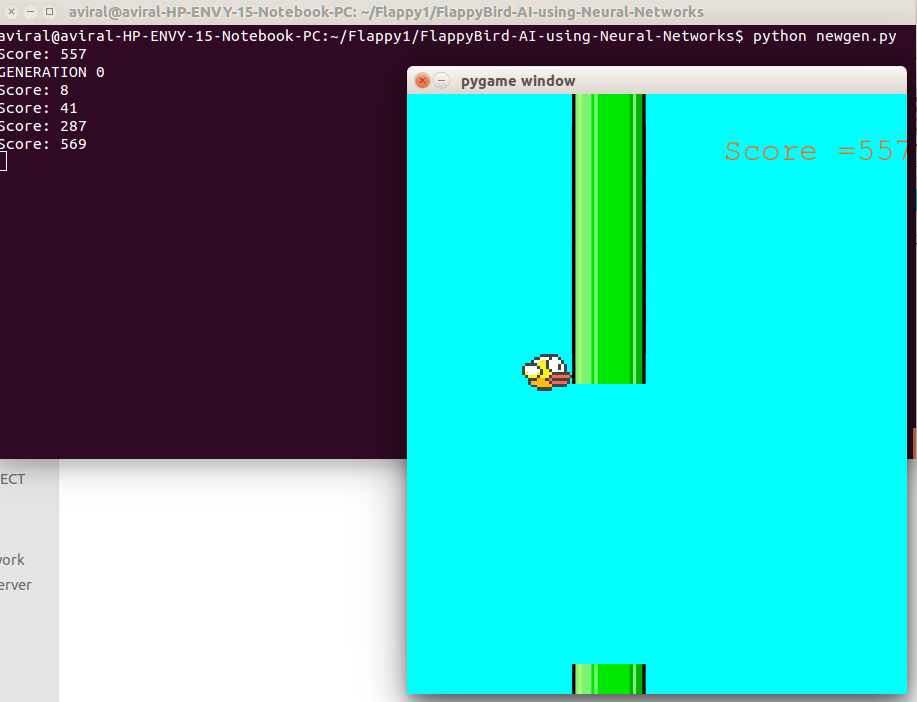
\includegraphics[width=0.65\vsize, angle = 0]{full.png} \\
\end{center}

\section{What we have done finally}
\begin{enumerate}
\item We have successfully made a working code implementing the Genetic Algorithm for solving the abocve stated problem, and tested it rigorously.
\item We have done extensive research about the Reinforcment Learning methodology of solving this problem, untill the 21st March deadline and hence mentioned all of it in the previous report, and written some small snippets of code for it (although they don't work properly)
\end{enumerate}

\section {Future Work}
\begin{enumerate}
    \item Genetic algorithm can be made more effective by changing the fitness parameter.
    \item With possibly more hidden layers, and different number of nodes in the neural net, the efficiency can be increased.
    \item Reinforcement learning technique can be applied to solve the same problem, although it's completely a different approach towards this problem. 
    \item Such ideas can also be applied to other games too.     
\end{enumerate}

\section{Conclusion}
We felt great while working on this project. We were quite fascinated by the fact that such simple "random" updates can develop such undefeatable game players. Also, the idea of evolution behind the Genetic Algorithms is also quite interesting.

\section{References}
\begin{enumerate}
\item A previous project done on same ideas : \url{http://cs229.stanford.edu/proj2015/362_report.pdf}
\item Base code for Flappy Bird Game : \url{https://github.com/TimoWilken/flappy-bird-pygame}
\item Theory about Genetic Algorithms : \url{https://www.doc.ic.ac.uk/~nd/surprise_96/journal/vol1/hmw/article1.html}
\item Theory about Genetic Algorithms : \url{http://theory.stanford.edu/~amitp/GameProgramming/AITechniques.html}
\item Examples on Genetic Algorithms :
\item \textbf{[Reference for Q-Learning]} Slides on Neural Networks RL : \url{http://web.mst.edu/ gosavia/neural networks RL.pdf}  
\item Wiki pages of the associated topics
\end{enumerate}

\end{document}